\documentclass[journal]{IEEEtran}
\usepackage[utf8]{inputenc}
\usepackage[official]{eurosym}
\usepackage{csquotes}
\usepackage{graphicx}

\usepackage{tikz}
\usetikzlibrary{automata,shapes,matrix,arrows,decorations.pathmorphing}

\usepackage{amsmath,amsfonts,amssymb}
\usepackage{bm}
\usepackage{mathtools}

\usepackage{lipsum}
% \usepackage[caption=false, font=footnotesize]{subfig}
\graphicspath{ {./graphics/} }
\hyphenation{op-tical net-works semi-conduc-tor}

\begin{document}
\title{Support Vector Machines: Theoretical Summary \& LIBSVM Experiments}% <-this % stops a space

\author{David~Kirby,~\IEEEmembership{Student Member,~IEEE}%
\thanks{The author is with the Department of Electrical and Computer Engineering, University of New Mexico, Albuquerque, NM 87131 USA (e-mail: davidkirby@unm.edu).}%
}

\maketitle
\begin{abstract}
    This paper describes the basic nomenclature and ideas behind risk, complexity as it applies to machine learning, the Vapnik--Chervonenkis theory and dimension, and support vector machines. It then goes into experiments showing how to use an SVM library; the chosen one is \texttt{libsvm}.
\end{abstract}
\begin{IEEEkeywords}
    Support Vector Machines, Statistical Learning Theory, VC Dimension, Risk, Complexity, Overfitting, LIBSVM
\end{IEEEkeywords}

\section{Introduction}

\IEEEPARstart{F}{or} students starting out in statistical data analysis, support vector machines (SVMs) offer an ideal introduction to the terminology and premises of machine learning through the use of foundational computer algorithms and optimization techniques. This paper strives to introduce the basic ideas behind SVMs, their practical applications, and then gives a series of experiments demonstrating the various features.

The state of the art for SVMs places them within the supervised learning subclass of machine learning~\cite{TDS}; however, SVMs can be adapted to unsupervised learning (clustering) and regression through the use of an expansive network of algorithms beyond the scope of this paper. The theoretical part of this paper describes the key features of SVMs including risk, complexity, the Vapnik–Chervonenkis theory and dimension, SVM criteria, the dual solution of the SVM, support vectors, and finally gives experiments performed in MATLAB. 

The algorithms used in the experiments are then compared to \texttt{svmpredict}, part of the open source \texttt{libsvm} library developed at the National Taiwan University and implements the SMO algorithm for kernelized support vector machines~\cite{LIBSVM}. For novelty, the paper also compares the MATLAB code and results with an open source Python implementation that uses \texttt{sklearn} and its SVM library.

The paper discusses the advantages and trade-offs of SVM, including but limited to working well with higher dimensions, are memory efficient, and can employ kernels, increasing their flexibility. Some of the trade-offs, however, include limited scalability and computationally expensive.

Machine learning can be divided into two main learning methods: supervised and unsupervised~\cite{Stat}. Supervised learning associates the input features of the training examples to the corresponding output labels as shown in Figure~\ref{fig:Machine}. While SVMs are flexible to enough to be used for classification or regression, this paper is focused primarily on classification. For this classification the author split the training data into binary clusters. The SVM is then designed to find the optimal hyperplane to separate these two classes defined by an equation and incorporating a structure and a training criterion. For the structure, one can use a family of linear functions: \( \hat{y_n} = \bm{\mathrm{w}}^\top\bm{\mathrm{x}}_n + b\). A criterion then needs to be chosen to optimize parameters \( \bm{\mathrm {w}} \). The simplest criterion in supervised learning is the minimization of the mean square error: \( e^2 = \left(y_n - \hat{y_n} \right) ^2 \). One can then use the law of large numbers to approximate.

\begin{figure}[ht]
    \centering
    \begin{tikzpicture}[scale=1.75,shorten >=4pt]
    \node (x4) at (1,1) {$x_4$};
    \node (x3) at (1,2) {$x_3$};
    \node (x2) at (1,3) {$x_2$};
    \node (x1) at (1,4) {$x_1$};
    \node[state] (+) at (3,2.5) {$+$};
    \node (y) at (5,2.5) {$\hat{y}=f(\text{\textbf{x}})$};
    \path[*->,font=\scriptsize]
    (x4) edge node[above]{$w_4$} (+)
    (x3) edge node[above]{$w_3$} (+)
    (x2) edge node[above]{$w_2$} (+)
    (x1) edge node[above]{$w_1$} (+);
    \path[->,font=\scriptsize]
    (+) edge node[above] {$Output$} (y);
    \end{tikzpicture}\vspace{-3em}
\begin{align*}
    \hspace{9em}
    \text{\textbf{x}} = \begin{Bmatrix}
    x_1\\
    \vdots\\
    x_D
    \end{Bmatrix},
    \text{\textbf{w}} = \begin{bmatrix}
    w_1\\
    \vdots\\
    w_D
    \end{bmatrix}
\end{align*}
\caption{Machine structure.}
\label{fig:Machine}
\end{figure}

\section{Theory}

\subsection{Risk: Empirical, Actual, and Structural}

The concepts of risk and empirical risk are two methods to measure the accuracy and precision of a particular algorithm. In machine learning, there are generally three different sets of risks: actual, structural, and empirical. Using these one can determine how poor or well a given set of data can be represented by an algorithm. One is also able to determine if the algorithm will underfit or overfit our data. Finally, it is possible to determine if the complexity of the model is too high or too low. Actual risk, or the probability of error during the test, cannot be directly computed as we do not have the data a priori; instead, we try to approximate the actual risk with the help of the structural and empirical risks. Structural risk is designed to ensure that our algorithm does not become too specialized on a training dataset. It compares the complexity of the machine against its success of fitting the data, this in turn reduces the likelihood of overfitting or underfitting. The empirical risk; however, uses a given or known set of training data to analyze the prediction efficacy of the machine, for example through the minimization of the mean square. The empirical risk is the average loss over the data points.

\subsection{Concepts of Complexity and Overfitting.}
In machine learning, complexity refers to the number of features and terms of a given model as well as its linearity. Complexity is directly proportional to the accuracy of the algorithm; however, increasing complexity can eventually reach a point of diminishing returns. When this happens, overfitting occurs and renders the model ineffective. Overfitting describes the condition when the algorithm classifies training data so closely that any test data could be misclassified. Over-complicating and overfitting create a highly specialized, but practically useless machine. We can reduce complexity by performing feature engineering and transforming data to extract valuable information.

\subsection{VC Dimension}

The Vapnik--Chervonenkis dimension was developed by Vladimir Vapnik and Alexey Chervonenkis during the 1960s--1990s as a statistical approach to classification problems. Used heavily in image classification, OCR, cancer prediction, and more, it is a binary classifier that attempts to maximize the separation between two classes of points. With regard to support-vector machines, the VC dimension determines the maximum number of vectors that can be shattered by a hyperplane and gives us a measure of the complexity of linear functions. If the VC dimension of an estimator is higher than the number of vectors to be classified, then the estimator is guaranteed to overfit if an empirical risk is minimized over the data, since all vectors will be correctly classified regardless of their statistical properties.

\subsubsection{VC theorem}

With the Vapnik--Chervonenkis theorem, we need to define the linear empirical risk as:
\begin{align}
	R_{emp}(\bm{\alpha}) &=\frac{1}{2N}\sum_{n=1}^{N} \bigm\lvert y-f(\bm{\mathrm{x}},\bm{\alpha}) \bigm\rvert
\end{align}
where \( f(\cdot) \) is defined so that the loss function \( \bigm\lvert y-f(\bm{\mathrm{x}},\bm{\alpha}) \bigm\rvert \) can only take the values of 0 or 1. Then, with the probability of \( 1-\eta \), the following bound holds:
\begin{align}
	R(\bm{\alpha}) \leq R_{emp}(\bm{\alpha}) + \sqrt{\frac{h(\log(2N/h)+1)-\log(\eta / 4)}{N}}
\end{align}
This is a bound on the risk with probability \( 1-\eta \), so it is therefore neither guaranteed nor dependent on the probability distribution. While the left side is not computable, the right one can be easily computed provided the knowledge of \( h \), where the second term of the right side is called the structural risk (\( R_s \)). The inductive \textit{Principle of Structural Risk Minimization} consists then of choosing a machine whose dimension \( h \) is sufficiently small, so that the bound on the risk is minimized. 

\subsection{SVM Criteria}

A support-vector machine constructs a hyperplane or set of hyperplanes in a high- or infinite-dimensional space, which can be used for classification, regression, or other tasks like outliers detection. To construct the optimal hyperplane, it takes the support of two other hyperplanes that are parallel and equidistant from it on either side. These two support hyperplanes lie on the most extreme points between the classes and are called support-vectors. This optimal hyperplane is called the maximum margin hyperplane. The distance between the support hyperplanes is called the margin and the goal of SVM then is to find the maximum margin.

\subsection{Dual Solution of the SVM}

The dual solution consists of minimizing the empirical risk and the structural risk through margin maximization as follows:
\begin{align}
	\text{minimize } &L_p(\bm{\mathrm{w}},\xi_n) = \frac{1}{2} \| \bm{\mathrm{w}} \|^2 +\ C \sum_{n=1}^{N} \xi_n\\
    \notag\text{subject to }&
        \begin{dcases}
            y_n\biggl(\bm{\mathrm{w}}^\top\bm{\mathrm{x}}_n + b\biggr) > 1 - \xi_n\\
            \xi_n \geq 0
        \end{dcases}
\end{align}
where \( C \) is a free parameter, \( p \) denotes primal, and \( \xi_n \) is  the distance a datapoint exceeds the respective support hyperplane towards the other class, hence \( \xi_n \geq 0\). The dual solution is designed to keep the objective function constant regardless of \( \bm{\mathrm{w}} \) and \( b \). Optimization is performed by computing the gradient with respect to \( \bm{\mathrm {w}} \), and then nullified. The minima is directly found by solving derivatives of the objective function; however, since there are constraints, we need to first take the Langrangian of the function to solve for the minima. Finally, solving for \( \bm{\mathrm {w}} \) results in Karush--Kuhn--Tucker conditions and creates a saddle point, i.e., a global maximum over the domain of the criteria and a global minimum over the multipliers.

The goal is to optimize the parameter \( C \). While there is no way that this parameter can be directly optimized (our professor and his colleagues have tried extensively), a reasonable way to find a good parameter is to do cross validation. We will see that cross validation is fundamental to making these machines work properly. It does this by putting a set of data for training and holding a set of data for validation. We train the machine with the training data and a given value of the free parameter \( C \) and then test with the validation set. Then change the value of the parameter and do it again, choosing the parameter that gives the minimum validation error.

There are many ways of doing this that are more or less efficient or that are more or less computationally heavy. If we do not have much data, then the validation might not work properly, so we need to find the most efficient possible validation. If we have a lot of data the same efficient validation procedure will take a lot of floating point operations. So the validation that we do depends on the conditions of our experiment. While this paper focuses on linear machines, it can be shown that this method can be used to pass from a linear machine to a non-linear one by using kernel tricks to change the number of dimensions of our data by passing the data through a non-linear transformation and the use of dot products.

\subsection{Support Vectors}

In support-vector machines, datapoints close to the hyperplane and satisfying certain conditions are called support vectors. If a datapoint is well within the boundary (support hyperplane), the penalizing factor \( \xi_n \) is 0. Otherwise, if the datapoint is on the other side, this factor \( \xi_n \) is equal to its distance between the datapoint and the support hyperplane, i.e., \( \xi_n \geq 0\) and \( \alpha_n = C \). If a sample is on the margin, \( 0 < \alpha_n = C \). Finally, if a sample is outside the margin, \( \xi_n = 0 \) and \( \alpha_n = 0 \).

\section{Experiments}

\subsection{Construction of a classifier with the model parameters.}

Using the parameters of the training, we constructed a machine that classifies the training data (Figure~\ref{fig:Param}) and compared our results with the ones of \texttt{svmpredict} (Figure~\ref{fig:svmPredict}). In order to find the equation of the classifier, we computed the primal parameter \( \bm{\mathrm{x}} \) from the dual ones \( \alpha_i \) and the data.

\begin{figure}[ht]
    \centering
    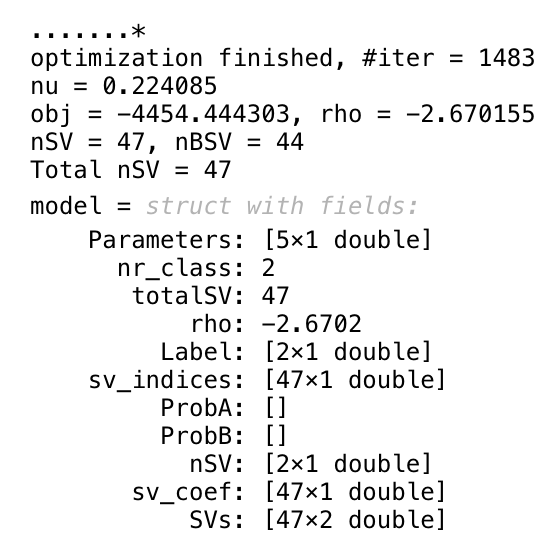
\includegraphics[width=0.8\linewidth]{modelParam.png}
    \caption{Construction of classifier.}
    \label{fig:Param}
\end{figure}

\begin{figure}[ht]
    \centering
    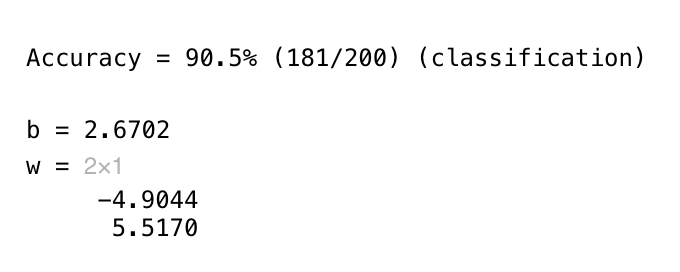
\includegraphics[width=0.8\linewidth]{svmpredict.png}
    \caption{Comparison with \texttt{svmpredict}.}
    \label{fig:svmPredict}
\end{figure}

\subsection{Graphical representation of an SVM.}

\subsubsection{Training matrix and training labels}

For this experiment, data vectors are defined as row vectors. Then, the input matrix must be \( N \times D\), where \( N \) is the number of training vectors (or patterns or instances) and \( D \) is the dimension of the space. The labels corresponding to the training vectors are defined as a column vector of scalars.
This simplistic example illustrates the data structure. We can generate a set of data by generating four Gaussians around four different centroids. Two are labeled with \(+1 \) and two with \( -1 \), \( + \) and \( \rm{o} \) respectively in Fig.~\ref{fig:data1} and Fig.~\ref{fig:data2}.

The SVM function needs to know what is the kind of SVM that will be run. To this end, the author constructed a string with the options. The main ones are:
\begin{align}
    \notag \texttt{-s} &\text{ svm type: set type of SVM (default 0)}\\
    \notag \texttt{-t} &\text{ kernel type: set type of kernel function (default 2)}\\
    \notag \texttt{-c} &\text{ cost: C-SVC, epsilon-SVR, and nu-SVR (default 1)}
\end{align}

An example can be run with the previous data and the Matlab line:
\begin{verbatim}
model=svmtrain(Y',X, '-s 0 -t 0 -c 100');
\end{verbatim}

This sentence means that we want to train an SVM using the previous data and that the SVM must be a linear (\texttt{-t 0}) classifier (\texttt{-s 0}), and with C = 100. In later experiments we will see that using the \texttt{-t 4} parameter we can pass a kernel to the SVM rather than passing data directly. This will expand our SVM capabilities and allow us to utilize polynomial, RBF, and Gaussian models.

\begin{figure}[ht]
    \centering
    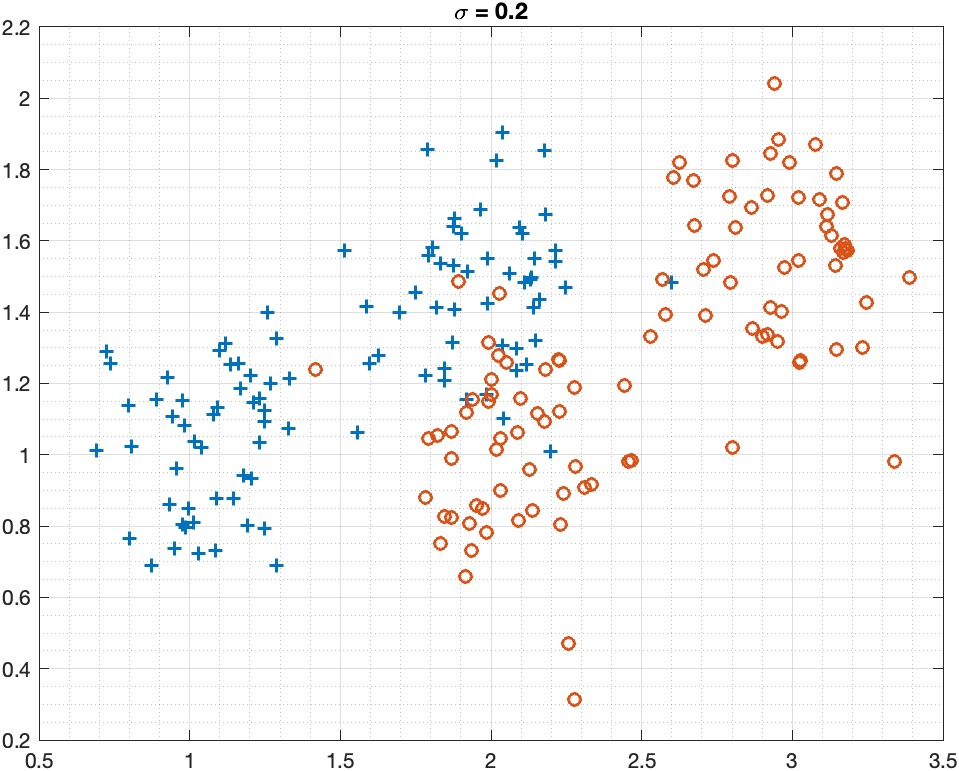
\includegraphics[width=\linewidth]{figure05.png}
    \caption{Fifty datapoints with \( \sigma = 0.2\).}
    \label{fig:data1}
\end{figure}

\begin{figure}[ht]
    \centering
    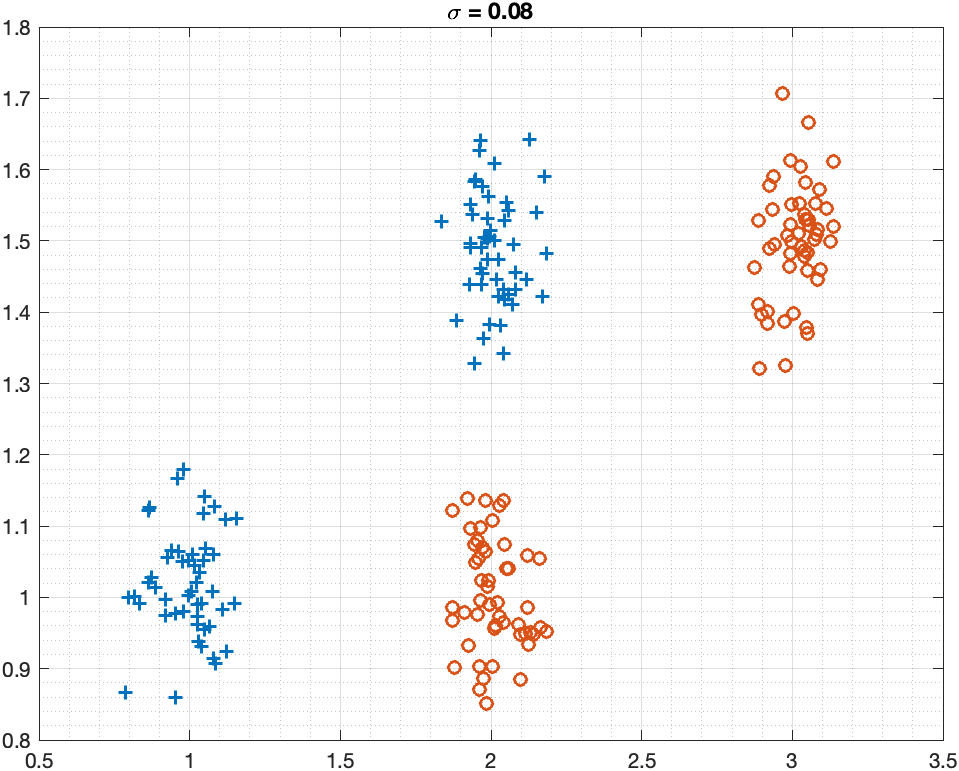
\includegraphics[width=\linewidth]{figure04.png}
    \caption{Fifty datapoints with \( \sigma = 0.08 \).}
    \label{fig:data2}
\end{figure}

Using the previous example, we plotted the separating line, the two margin lines and the support vectors resulting of the SVM training. the author did it for a smaller value and a higher value of parameter `sigma' of the data generating code.

To better see what was happening when plotting, the author increased N from 10 to 50. the author also chose to vary \( \sigma \) from 0.2 to 0.02 to get a better idea for what is being changed. As is evidenced by the plots in Figure~\ref{fig:data1} and Figure~\ref{fig:data2}, \( \sigma \) determines how separated the data is from the center. To this end, the author can think of \( \sigma \) as the standard deviation.

\begin{figure}[ht]
    \centering
    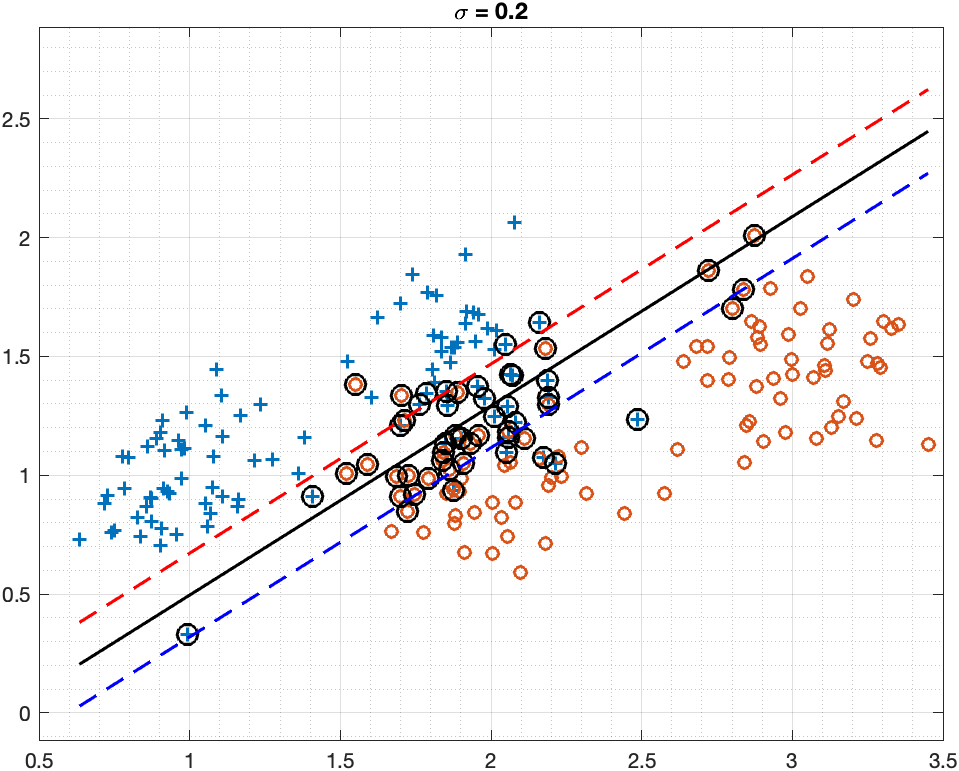
\includegraphics[width=\linewidth]{figure02.png}
    \caption{Support-vectors for \( \sigma = 0.2\).}
    \label{fig:SVM-0.2}
\end{figure}

\begin{figure}[ht]
    \centering
    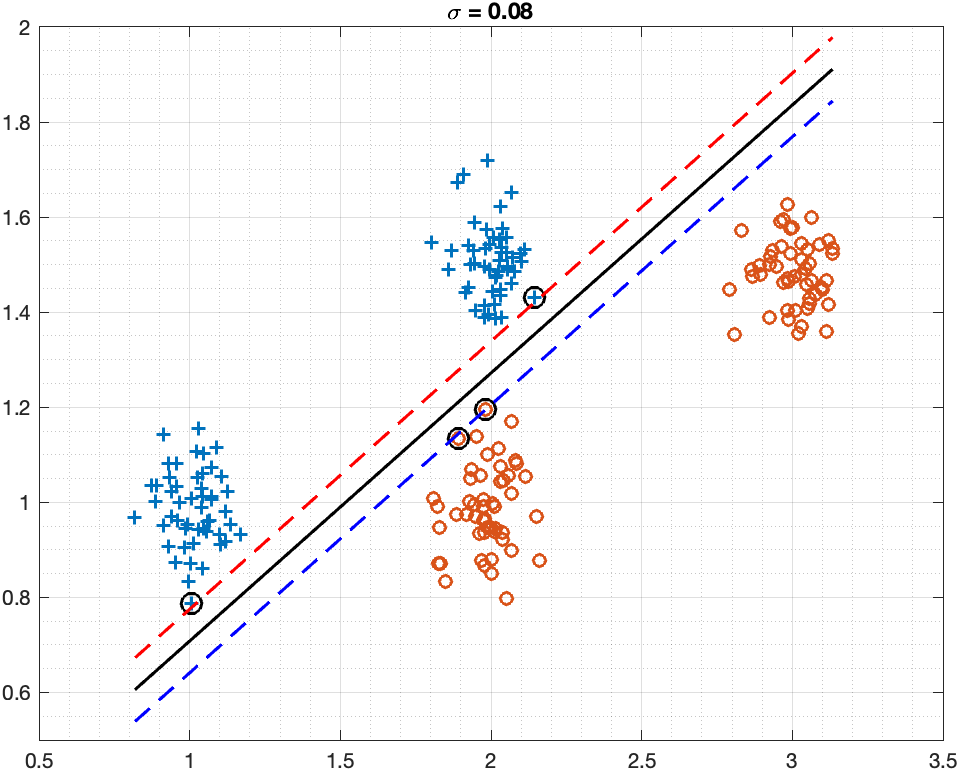
\includegraphics[width=\linewidth]{figure03.png}
    \caption{Support-vectors for \( \sigma = 0.08\).}
    \label{fig:SVM-0.08}
\end{figure}

\subsection{Estimating the structural risk.}

The objective of this experiment was to draw a plot of the actual risk ($R(\alpha )$) and the empirical risk $R_{emp} (\alpha )$, considering a space of 10 dimensions and a set of data that can be represented and classified in a subspace of only 3 dimensions. Thus, a linear classifier of $h=4$ was sufficient to properly solve the classification problem.

It first generates eight points describing a cube of dimension \( \sigma \). Four of the points are at one side of the plane described by the equation \( \Pi = \bm{\mathrm{w}}^\top\bm{\mathrm{x}} + b \) where \( \rm w_i = 1/\sqrt{10} \) and \( b = 0 \), at a distance \( \sigma /2 \), and they are labeled with \( -1 \). The other four are at the other side of the plane and they are labelled as \( +1 \).

Each pattern is generated by choosing at random one of the eight points and then adding a ten-dimensional Gaussian noise of standard deviation \( 0.2 \sigma \). It is straightforward to prove that hyperplane  is the optimal separating hyperplane in a Bayesian sense, that is, it will produce the minimum possible actual risk.

\begin{figure}[ht]
    \centering
    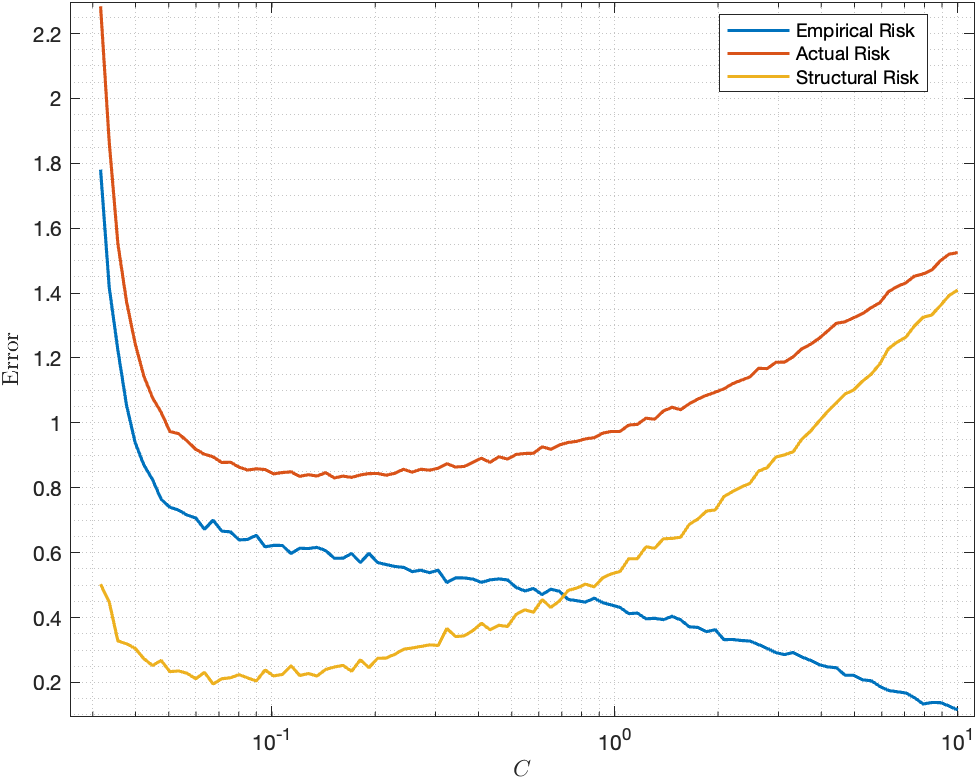
\includegraphics[width=0.5\textwidth]{figure01.png}
    \vspace{-1em}\caption{Plot of actual, empirical, and structural risks.}
    \label{fig:Risks}
\end{figure}

\section{Discussion}

This paper was designed to describe the basic nomenclature and ideas behind risk, complexity as it applied to machine learning, the Vapnik--Chervonenkis theory and dimension, and support vector machines. It then went into experiments showing how to use an SVM library; namely \texttt{libsvm}. The author would like to further pursue converting this code into Python and retrying the experiments using open source methods and \texttt{libsvm}. The author used a Macbook with ARM processor for all experiments; therefore, MATLAB was run under Rosetta 2 ISA emulation. The author would like to try running the experiments under a native language (i.e., Python) to test speed performance.

\section*{Acknowledgment}
The author would like to thank the University of New Mexico for the generous access to research material, as well as Dr. Manel Martínez-Ramòn for the opportunity to explore Machine Learning and Support Vector Machines.

\begin{thebibliography}{6}
\bibstyle{IEEEtran}

\bibitem{Vapnik1}
V.~Vapnik, A.~Chervonenkis and N.~Moskva, \enquote{Theory of Pattern Recognition,} \textit{Statistical Problems of Learning}, 1974.

\bibitem{TDS}
S.~Dobilas, \enquote{SVM Classifier and RBF Kernel -- How to Make Better Models in Python,} \emph{Toward Data Science}, Jan. 16, 2021. [online] [Accessed: Jan. 16, 2021].

\bibitem{LIBSVM}
C.~C.~Chang and C.~J.~Lin, \enquote{LIBSVM: A Library for Support Vector Machines,} \textit{Association for Computing Machinery}, 2011, Vol. 2,
Issue \#3, [online] [Accessed: https://doi.org/10.1145/1961189.1961199].

\bibitem{Tutorial}
C.~J.C.~Burges, \enquote{A Tutorial on Support Vector Machines for Pattern Recognition,} \textit{Data Mining and Knowledge Discovery 2}, 1998, pp. 121-167.

\bibitem{Stat}
T.~Hastie, R.~Tibshirani and J.~Friedman, \textit{\enquote{The Elements of
Statistical Learning: Data Mining, Inference, and Prediction,}} 2nd ed., Springer, 1998.

\end{thebibliography}

\end{document}
